\chapter[Fitting]%
{Optimisation and Parameters Fitting}
\label{ch:three}
\chapterquote{"...if the universities will not study useless subjects, who will?"}{G. F. Fitzgerald, Nature, 45/46, 392 (1892)}
%
\section{Fitting procedure}
\par{The problem of fitting, or nonlinear least square problem, is fundamental in
many fields. The problem can be very easily written as an optimisation problem
with an objective function}
\be
f(\theta)=\sum_{l}(y_l-F(x_l,\theta))^2
\ee
where $x_l$, $y_l$ are given data vectors and $\theta$ is a parameter
vector. Usually under certain assumptions the most likely values of $\theta$
represents the global optimiser. The ideal value of $f(\theta_{opt})=0$, but
usually a small value for the objective function is accepted. Choosing norm-2
as definition for $f(\theta)$ could be considered totally arbitrary.
\par{So the optimisation problem becomes}
\begin{equation*}
\textrm{Find} \min f(\theta)
\end{equation*}
\begin{equation*}
s.t.\quad\theta\in\boldsymbol{\theta}
\end{equation*}
where
$\boldsymbol{\theta}=[\underline{\theta},\overline{\theta}]=\{\theta\in\mathbb{R}^n|\underline{\theta}\leq\theta\leq\overline{\theta}\}$
is bounded or unbounded box in $\mathbb{R}^n$
($\underline{\theta}\in(\mathbb{R}\cup\{-\infty\})^n$ and
$\overline{\theta}\in(\mathbb{R}\cup\{+\infty\})^n$).
\par{To solve this problem there are two main categories of methods: complete
methods and incomplete methods. The complete methods are very sophisticated and
generally, there are mathematical proofs beyond them that assure us the
convergence. Often these methods requires a large number of function
evaluations and theirs derivatives. On the other hand, incomplete methods do
not have usually mathematical proofs beyond to sustain their use. The main
advantages of latter methods are: they can be cheap in terms of number of
function evaluations; they are very easy to be implemented; they can not
require derivatives of the cost function. An excellent up-to-date review about
optimisation is \citep{Neumaier03}.}
\par{For our fitting problem we choose to implement three incomplete methods:
Simplex, Simulated Annealing and a hybrid method Simplex-Simulated
Annealing. In our case the vector $y_l$ represents a set of \emph{ab initio}
total energies and $F(x_l,\theta)$ represents the total energy computed with
our tight binding model.}
\section{Simplex}
\par{Since its publication in 1965, Nelder-Mead simplex algorithm \citep{Nelder65}
has become one of the most used methods for nonlinear optimisation (this
algorithm should not be confused with the Simplex algorithm of Dantzig\marginpar{citation needed}). Many
versions of the simplex were implemented since its appearance. All of them
share more or less the same advantages and disadvantages. An excellent
discussion about simplex with pro's and con's is \citep{Lagarias98}.}
\par{The simplex method attempts to minimize a real function maintaining at each
step a nondegenerate simplex (a geometric figure in $n$ dimensions with non-zero
volume that is the convex hull of $n+1$ vertices).}
\par{Each iteration of the algorithm starts with a simplex specified by its $n+1$
vertices and function values. One or more test points are computed and
iteration finish with a new simplex which satisfies some descent conditions.}
\par{Four scalar parameters determine the way in which new points are
computed. Coefficient of reflection, $\rho$, expansion, $\chi$, contraction,
$\gamma$, and shrinkage, $\sigma$ satisfy}
\be
\rho>0,\quad \chi>1,\quad \chi>\rho,\quad 0<\gamma<1 \quad \text{and}\quad 0<\sigma<1
\ee
\par{Condition $\chi>\rho$ was not stated explicitely in the original paper, but it
is implicitly used. These parameters have ``universal'' choices in standard use
of algorithm}
\be
\rho=1;\quad \chi=2;\quad \gamma=\frac{1}{2}; \quad \text{and}\quad \sigma=\frac{1}{2}
\ee
\par{To the original implementation from \citep{Press07} we added constraints. If the new
vertex generated in a test step is outside the box an infinite value is
assigned to the objective function. In this way the simplex contracts again in
the box. To improve the quality of solution after the algorithm ``claims'' a
minimum a restart is done until in $m$ successive restarts the difference
between the best solution and the claimed solution is not great than the
tolerance. Figure \gref{simplex} presents the algorithm in a pseudocode
format.}\marginpar{the pseudocode should be rewritten with algo class}
\begin{figure}[!htb]
\begin{verbatim}
Step 1: compute psum
Step 2: find ilo, ihi, inhi (best, worst and next worst points)
Step 3:
  compute rtol
  if rtol<ftol then
  best point found ilo
  else
   if current_iter < max_iter then
     ytry: expand around ihi fact -1
     if ytry <=y(ilo) then
       ytry: expand around ihi fact 2
       else if ytry >= y(inhi) then
              ysave=y(ihi)
              ytry: expand around yhi fact 0.5
                if ytry >= ysave then
                   contract around ilo
                   goto step 1
                endif
            else
             goto step 2
            endif
     endif
   endif
  endif
\end{verbatim}
Compute psum step: $psum(i)=\sum_{j=1}^{ndim+1}p(j,i)$\\
Contract around ilo step: $p(i,j)=\frac{1}{2}\sum_{j=1, i\neq ilo}^{ndim}(p(i,j)+p(ilo,j))$\\
Expand around ii fact fac\\
$fac1=(1-fac)/ndim$ $fac2=fac1-fac$\\
$ptry(j)=fac1*psum(j)-p(ii,j)*fac2$\\
if $funk(ptry(j))<y(ii)$ then $p(ii,j)=psum(j)-p(ii,j)+funk(ptry(j))$
\caption{Simplex pseudocode}
\label{simplex}
\end{figure}
\section{Simulated Annealing (SA)}
\par{The idea beyond SA is the fact that heating (annealing) and slow cooling of a
metal brings it into a more uniformly crystalline state that is believed to be
the state where the free energy of bulk matter takes its global minimum. The
role of ``temperature'' is to allow the configurations to reach a higher
energy states with the probability given by Boltzmann's law in an original
version. The initial algorithm was proposed by Kirkpatrick
\citep{Kirkpatrick83} based on Metropolis Monte Carlo integration algorithm
\citep{Metropolis53}. The formal description of the algorithm is given in Figure
\gref{SA} in pseudocode version.}\marginpar{the pseudocode should be rewritten with algo class}
\begin{figure}[!htb]
\begin{verbatim}
!factor - annealing temperature reduction factor
!ntemps - number of temperatures step to try
!nlimit - number of trials at each temperature
!glimit - number of succesful trials (or swaps)

initialize temperature
do i=1,ntemps
   temperature=factor*temperature
   do j=1,nlimit
      try swapping a random pair of points
      delta=curent_cost-trial_cost
      if delta>0 then
         make the swap permanent
         increment good_swaps
      else
         p = random number in [0,1]
         m=exp(delta/temperature)
         if p < m then      !Metropolis criterion
            make the swap permanent
            increment good_swaps
         endif
      endif
      exit when good_swaps > glimit
   enddo
enddo
\end{verbatim}
\caption{SA pseudocode}
\label{SA}
\end{figure}
\par{The temperature schedule it is of a crucial importance and the success of the
method is based on it.
Boltzmann annealing consists in reducing the temperature in step k according
to a logarithmic law}
\be
T(k)=\frac{T_0}{\ln k}
\ee
with $T_0$ ``large enough''. Cauchy annealing or fast annealing is
\be
T(k)=\frac{T_0}{k}
\ee
\par{Other schedules used in practice}
\be
\label{oscheldue}
T_{k+1}=cT_k\quad 0<c<1
\ee
\begin{equation*}
T_k=T_0\exp{(c-1)k}
\end{equation*}
\begin{equation*}
T_{k+1}=T_k-T_0\frac{\ln k_0}{k(\ln k)^2} \quad k_0\text{ a starting index}
\end{equation*}
\par{Usually the option for one or other program is determined by the class of
problem that we study. Tuning of method is crucial for the success. An
interesting discussion about tuning and schedules could be found in
\citep{Ingber93}\marginpar{add the other papers}.}
\par{Our implementation of SA is based on schedule from \gref{oscheldue}
in the form suggested by Corana \emph{et al.} \citep{Corana87}.}
\par{Even if the method is proved to be convergent in a probabilistic sense it could
be very slow. The convergence could be improved by making ad hoc
enhancements.}
\par{The ad hoc improvement suggested by Corana's implementation is the existence
of a variable step length vector.}
\be
x^{\prime}=x_i+rv_{n_k}e_k
\ee
where $r$ is a random number in $[-1,1]$, $v_{n_k}$ is the $k$-th component of
step length vector and $e_k$ is the $k$-th elementary vector, $x_i$ is the
initial point.
\par{In addition a recipe is provided to vary the step length vector in such a way
to maintain the average of accepted moves about $1/2$. }
\section{Simplex-Simulated Annealing (SSA)}
\par{The method is a combination of a ``shaken'' simplex with an annealing
schedule. The idea is suggested in \citep{Press07}. In SA algorithm the Metropolis step
is replaced by a subtle modified simplex. An positive random logarithmic value
proportional with temperature is added to every stored value associated with a
vertex and a similar random value is subtracted from the value associated
with a trial vertex.}
\par{In the limit $T\rightarrow 0$ we obtain the normal simplex algorithm. The
randomness gives us exactly the same behaviour as the Metropolis
algorithm. Again the schedule program of cooling it is crucial for the
convergence of the problem. However the test functions investigated suggested
that the problem of temperature schedule is not as critical as in the case of
the native SA algorithm.}
\par{To improve convergence of the algorithm we customised it a little bit. After
the SSA claims a point we start a simplex optimisation to check the
claim. Again the termination condition is a multi-step one. }
\section{Tests}
\par{The next 8 test functions were investigated in 2 and 10 dimensions. The
results are gathered in Table \gref{tabletest}.}
\par{Few observations about the Table \gref{tabletest} are necessary: $T_{CPU}$ is
in seconds as given by the function \verb|cpu_time| (standard in Fortran
95). Column \emph{hits} represents the number of success claims out of 2000,
for 2 dimensional test and out of 10000 for 10-dimensional tests. \emph{hits1}
represents the success count for SSA before calling the added simplex step and
\emph{hits2} represents the final number of successful claims. The tolerance
was the same for all the test $1e-8$. No special tuning was carried, so the results could be improved. That is the situation
for Rastrigin and Rosenbrock functions in 10-dimensions. The zero from column
\emph{hits1} from Ackley and Schwefel means that no reasonable precision was
meet. As a general conclusion we can not say that one or other method is
successful or not. The employment of them should be done only after a careful
study of the problem. In all pictures the orientation of the surface in
indicated by a coloured system of axes (the legend to it is $xyz\rightarrow RGB$).}
%
\par{Levy No 3 function, see figure \gref{levy3},  has 18 global minima at
$-186.73090$  (2 dimensions) and about 760 local minima in the box
$-10.0\leq x_i \leq 10.0$ $i=\overline{1,2}$}
%
\be
\label{levy3f}
f(x)=\sum_{i=1}^{5}i\cos[(i+1)x_1+i]\sum_{j=1}^{5}j\cos[(j+1)x_2+j]
\ee
%
\begin{figure}[tb]
\begin{center}
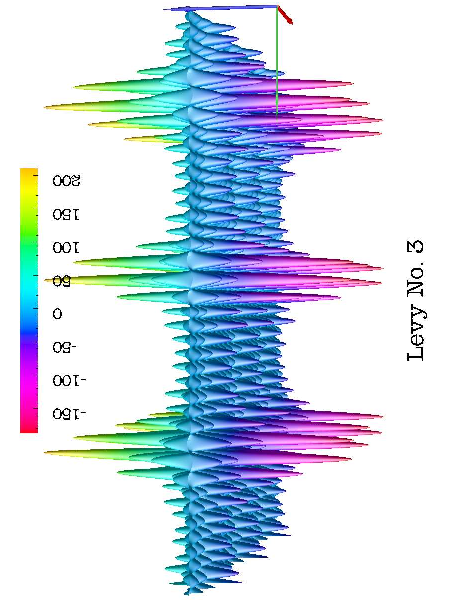
\includegraphics[width=0.5\textwidth,angle=-90]{figures/levy3}
\caption{\label{levy3} Levy No 3  \gref{levy3f}}
\end{center}
\end{figure}
%
\begin{figure}[!htb]
\begin{center}
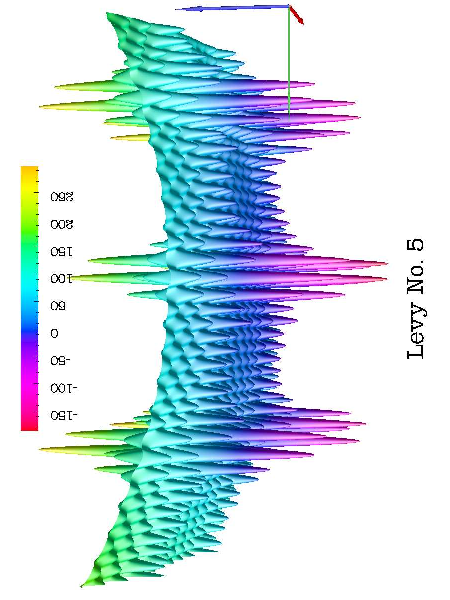
\includegraphics[width=0.5\textwidth,angle=-90]{figures/levy5}
\caption{\label{levy5} Levy No 5  \gref{levy5f}}
\end{center}
\end{figure}
\par{Levy No 5 function, see figure \gref{levy5},  has a global minimum
$-186.73090$  and about 760 local minima (2 dimensions) in the box
$-10.0\leq x_i \leq 10.0$ $i=\overline{1,2}$}
%
\be
\label{levy5f}
f(x)=\sum_{i=1}^{5}i\cos[(i+1)x_1+i]\sum_{j=1}^{5}j\cos[(j+1)x_2+j]+(x_1+1.42513)^2+(x_2+0.80032)^2
\ee
%
%
\par{Levy No 8 function, see figure \gref{levy8},  has a global minimum
$0$ at $(0,0,0 ...)$ in the box
$-10.0\leq x_i \leq 10.0$ $i=\overline{1,n}$}
%
\be
\label{levy8f}
f(x)=\sin^2(\pi y_1)+\sum_{i=1}^{n-1}(y_i-1)^2[1+10\sin^2(\pi y_{i+1})]+(y_n-1)^2
\ee
where $y_i=1+\frac{x_i-1}{4}$\\
%
\begin{figure}[!htb]
\begin{center}
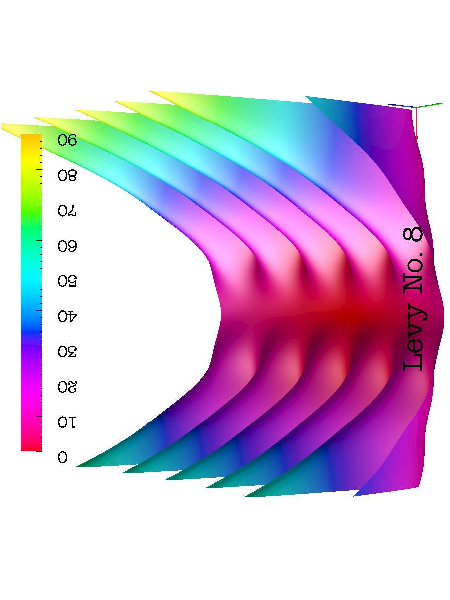
\includegraphics[width=0.5\textwidth,angle=-90]{figures/levy8}
\end{center}
\caption{Levy No 8  \gref{levy8f}}
\label{levy8}
\end{figure}
%
\begin{figure}[!htb]
\begin{center}
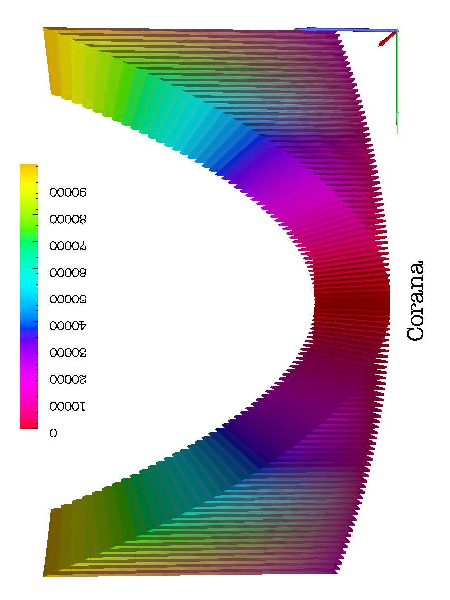
\includegraphics[width=0.5\textwidth,angle=-90]{figures/corana}
\caption{Corana  \gref{coranaf}}
\label{corana}
\end{center}
\end{figure}
%
\par{Corana function, proposed in \citep{Corana87} has a global minimum $0$ at $(0,0,0 ...)$ in the box
$-1000.0\leq x_i \leq 1000.0$ $i=\overline{1,n}$}
%
\be
\label{coranaf}
f(x)=\sum_{i=1}^n\left\{\begin{array}{ll}
(t_i\textrm{sgn}({z_i})+z_i)^2cd_i&\textrm{if }|x_i-z_i|<|t_i|\\
d_ix_i^2&\textrm{otherwise}
\end{array}\right.
\ee
where $z_i=\lfloor |x_i/s_i|+0.49999\rfloor\textrm{sgn}(x_i)s_i$, $s_i=0.2$,
$t_i=0.05$, $d_i=(1,1000,10,100, ...)$, $c=0.15$, $s_i,t_i,d_i$ repeated in cycles of 4, $c$ is a coefficient
defined in such a that \gref{coranaf} defines a paraboloid with axis parallel
to the coordinates, and a set of holes ($\lfloor x\rfloor$ is floor function
giving largest integer less than or equal to $x$), see Figure \gref{corana}.
\par{Rosenbrock function, see figure \gref{rosenbrock},  has a global minimum 0 at
$(1,1,1,...)$ in the box $-2.048\leq x_i \leq 2.048$ $i=\overline{1,n}$}
\be
\label{rosenbrockf}
f(x)=\sum_{i=1}^{n-1}100(x_{i+1}-x_i^2)^2+(1-x_i)^2
\ee
\begin{figure}[!htb]
\begin{center}
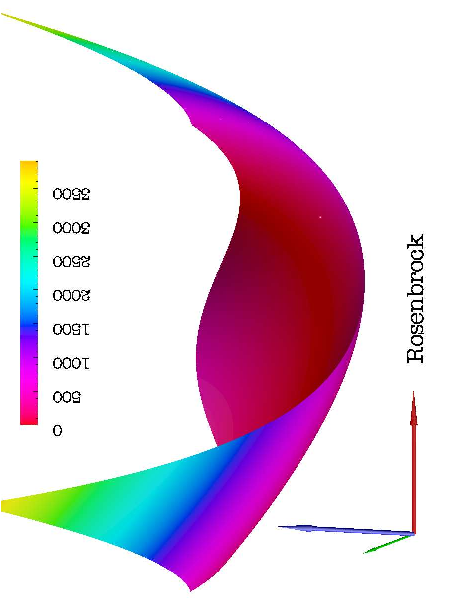
\includegraphics[width=0.5\textwidth,angle=-90]{figures/rosenbrock}
\end{center}
\caption{Rosenbrock  \gref{rosenbrockf}}
\label{rosenbrock}
\end{figure}
\begin{figure}[tb]
\begin{center}
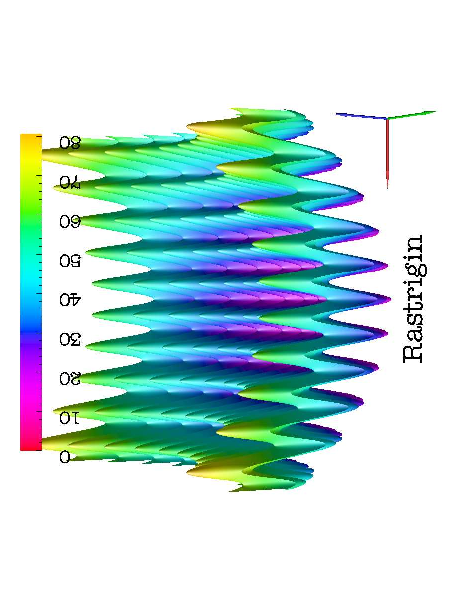
\includegraphics[width=0.5\textwidth,angle=-90]{figures/rastrigin}
\end{center}
\caption{Rastrigin  \gref{rastriginf} }
\label{rastrigin}
\end{figure}
\par{Rastrigin function, see figure \gref{rastrigin},  has a global minimum 0 at $(0,0,0,...)$ in the box
$-5.12\leq x_i \leq 5.12$ $i=\overline{1,n}$}
\be
\label{rastriginf}
f(x)=10n+\sum_{i=1}^{n}x_i^2-10\cos(2\pi x_i)
\ee
%
\par{Schwefel (Sine root) function, see figure \gref{schwefel},  has a global
minimum 0 at $(c,c,c,...)$ $c=420.9687464$ in the box
$-500\leq x_i \leq 500$ $i=\overline{1,n}$}
\be
\label{schwefelf}
f(x)=418.982887272433n-\sum_{i=1}^{n}x_i\sin(\sqrt{|x_i|})
\ee
\begin{figure}[!htb]
\begin{center}
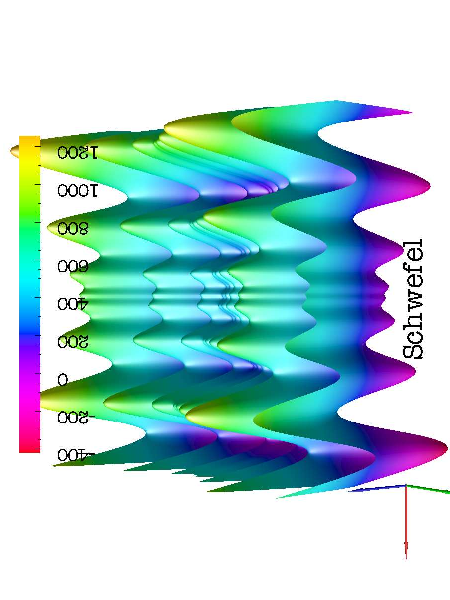
\includegraphics[width=0.5\textwidth,angle=-90]{figures/schwefel}
\end{center}
\caption{Schwefel  \gref{schwefelf}}
\label{schwefel}
\end{figure}
%
\begin{figure}[!htb]
\begin{center}
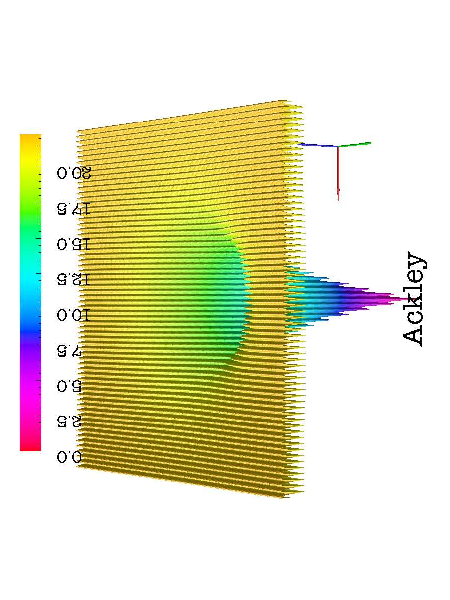
\includegraphics[width=0.5\textwidth,angle=-90]{figures/ackley}
\end{center}
\caption{Ackley  \gref{ackleyf}}
\label{ackley}
\end{figure}
\par{Ackley function, see figure \gref{ackley},  has a global minimum 0 at
$(0,0,0,...)$ in the box $-32.768\leq x_i \leq 32.768$ $i=\overline{1,n}$}
%
\be
\label{ackleyf}
f(x)=20+e-20\exp{\biggl[-0.2\sqrt{\frac{1}{n}\sum_{i=1}^{n}x_i^2}\biggr]}-\exp{\biggl[\frac{1}{n}\sum_{i=1}^{n}\cos(2\pi x_i)\biggr]}
\ee
%
%
\begin{table}[!htb]
\caption{Tests results}
\label{tabletest}
%\begin{spacing}{1.0}
\begin{center}
\begin{tabular}[h]{|l|r|r|r|r|r|r|r|}
\hline
Algorithm & \multicolumn{2}{|c|}{Simplex} & \multicolumn{2}{|c|}{SA} &
\multicolumn{3}{|c|}{SSA}\\
\hline
Function& $T_{CPU}$ & Hits & $T_{CPU}$ & Hits& $T_{CPU}$ & Hits1 & Hits2\\
\hline
\hline
\multicolumn{8}{|c|}{2 dimensions}\\
\hline
Levy no 3&5.56&1922&32.44&2000&74.70&1332&1999\\
\hline
Levy no 5&5.68&810&34.07&816&52.41&567&729\\
\hline
Levy no 8&4.69&2000&21.55&2000&66.97&983&2000\\
\hline
Corana&3.78&2000&24.17&2000&19.69&52&2000\\
\hline
Rosenbrock&4.28&2000&19.07&1995&53.06&896&2000\\
\hline
Rastrigin&4.31&988&14.66&1441&25.71&29&1348\\
\hline
Schwefel&4.56&1033&21.67&1983&39.56&636&1817\\
\hline
Ackley&5.47&2000&23.15&2000&97.09&1743&2000\\
\hline
\hline
\multicolumn{8}{|c|}{10 dimensions}\\
\hline
Levy no 8&568.76&9985&1322.59&10000&1884.03&1714&9988\\
\hline
Corana&495.86&9888&1186.01&9987&913.12&0&9895\\
\hline
Rosenbrock&313.29&8133&713.00&0&1690.20&7181&8246\\
\hline
Rastrigin&566.8626&2338&927.06&0&1581.78&0&2428\\
\hline
Schwefel&625.98&2879&1138.84&627&1598.23&0&2856\\
\hline
Ackley&499.62&9992&1005.59&10000&938.98&0&9989\\
\hline
\hline
\end{tabular}
\end{center}
%\end{spacing}
\end{table}
%
\section{Tight binding $N-H$, $N-N$ parameters}
\par{The fitting procedure described above was employed to solve the problem of
fitting the parameters for $N-H$ and $N-N$ bonds in a $NH_3$ and $N_2$
molecules. The parameters are from GSP-like scheme. The ``exact'' data are
represented by a hybrid DFT total energy curves. The basis set used to obtain them
was $6.31G(d,p)$ with the B3LYP functional. For $N_2$ the curve represents total energy vs $N-N$ bond length. For $NH_3$
two curves are investigated one is total energy vs $N-H$ bond length and the
second represents total energy vs $\theta$, where $\theta$ is defined as the
angle between $N-H$ bond direction and $C_3$ axis of symmetry, we refer about
the latter as ``umbrella'' curve. Table \gref{tablen2} summarise the parameters
for $N-N$ in $N_2$ molecule and Figure \gref{fitn2} shows the fit using our three
methods. The $N-H$ parameters for both modes are given in Table \gref{tablenh3}
and the fits are shown in figures \gref{fitnh3} and \gref{fitnh3um}.The zero
of energy is set to total energy of equilibrium geometry provided by hybrid
DFT calculations and the units are eV. The great majority of parameters from from Tables
\gref{tablen2} and \gref{tablenh3} lacks the physics due to the almost free
fitting strategy carried.}
\par{With the set of parameters provided by SSA method for $N-H$ bond we carried a
geometry optimisation using TDTB+UJ. The bond length was reproduced up to 0.008
{\AA} ($1.010$ {\AA} instead of $1.018$ \AA), but the bond angle was
underestimated ($88.7^\circ \approx 90^\circ$ instead of $105.7^\circ$). An
improvement could come adding $d$-orbitals, but we have not investigated
this option, yet. This lack of transferability of parameters
could come from the lack of physical insight put into the parameters
constraints. Figures \gref{spacenh3} and \gref{umbnh3} show us the surface of
the objective function in the space of two parameters, that we think could be
very important for the transferability of the model, $\epsilon_s$ (x
direction) and $\epsilon_p$ (y direction). The scanning is done in the box
$[-10.0,10.0]$ in an equal spaced grid of $201\times 201$. }
%
\begin{figure}[!htb]
\begin{center}
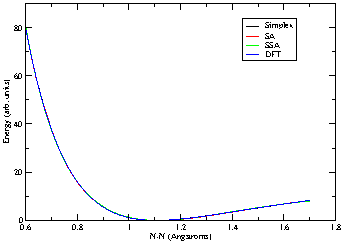
\includegraphics[width=0.75\textwidth]{figures/n2}
\end{center}
\caption{$N_2$ Energy fit}
\label{fitn2}
\end{figure}
%
\begin{figure}[!htb]
\begin{center}
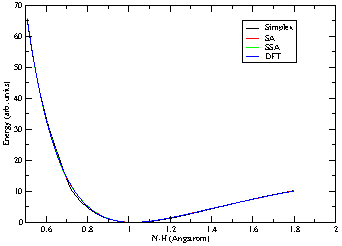
\includegraphics[width=0.75\textwidth]{figures/nh3}
\end{center}
\caption{$NH_3$ Energy fit}
\label{fitnh3}
\end{figure}
%
\begin{figure}
\begin{center}
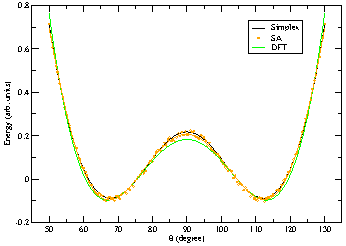
\includegraphics[width=0.75\textwidth]{figures/nh3u}
\caption{$NH_3$ ``Umbrella'' Energy fit}
\label{fitnh3um}
\end{center}
\end{figure}
%
\begin{figure}
\begin{center}
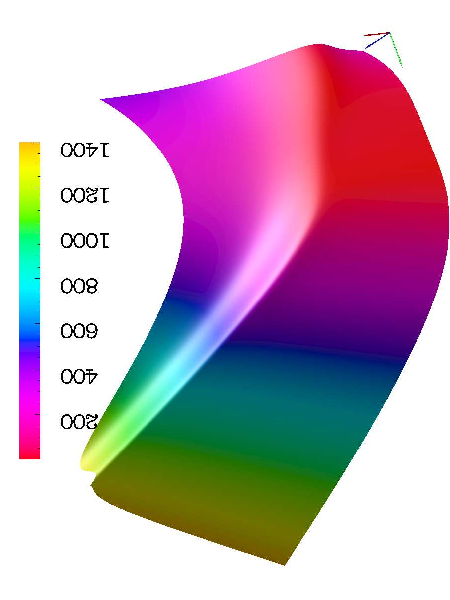
\includegraphics[width=0.5\textwidth,angle=-90]{figures/obj}
\caption{$NH_3$ Energy in $\epsilon_s$, $\epsilon_p$ space}
\label{spacenh3}
\end{center}
\end{figure}
%
\begin{figure}[!htb]
\begin{center}
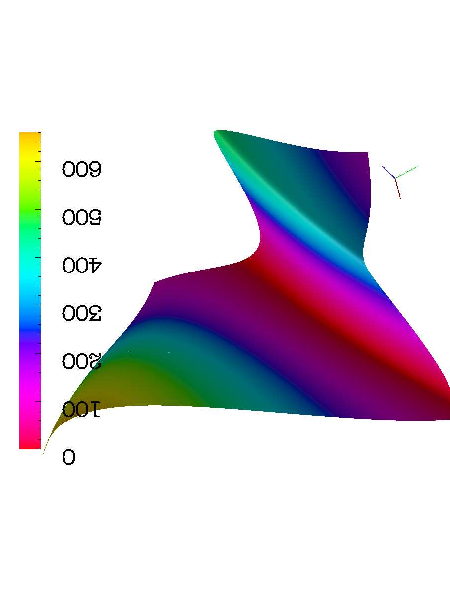
\includegraphics[width=0.5\textwidth,angle=-90]{figures/umbobj}
\caption{$NH_3$ ``Umbrella''Energy in $\epsilon_s$, $\epsilon_p$ space}
\label{umbnh3}
\end{center}
\end{figure}
%
%
%
\begin{table}[!thb]
\caption{$N-N$ $N_2$ parameters}
\label{tablen2}
\begin{center}
\begin{tabular}{|l|r|r|r|}
\hline
Parameter & Simplex & SA & SSA\\
\hline
\hline
$\epsilon_s$&-1.1952&-5.6667&-3.0500\\
\hline
$\epsilon_p$&4.4639&9.9550&1.0029\\
\hline
$\phi_0$&5.7837&8.8705&9.9991\\
\hline
$r_c$&1.3000&1.6913&1.5844\\
\hline
$n$&0.7689&1.5224&1.0531\\
\hline
$n_c$&2.5430&4.7195&3.8904\\
\hline
$d_0$&1.7141&1.1355&1.4432\\
\hline
$d_c$&1.9694&2.0393&1.9867\\
\hline
$m$&2.3991&3.5303&2.9362\\
\hline
$m_c$&5.5447&2.9813&8.2075\\
\hline
$ss\sigma$&8.5856&-9.2457&2.6236\\
\hline
$sp\sigma$&-8.3785& 0.8549&4.8730\\
\hline
$pp\sigma$&9.9148&4.6912&9.9552\\
\hline
$pp\pi$&9.5853&-2.7325&-3.9943\\
\hline
\end{tabular}
\end{center}
\end{table}
%
\begin{table}[!htb]
\caption{$N-H$ $NH_3$ parameters}
\label{tablenh3}
\begin{center}
\begin{tabular}{|l|r|r|r|r|r|r|}
\hline
Parameter &\multicolumn{3}{|c|}{E vs $N-H$}&\multicolumn{3}{|c|}{``Umbrella''}\\
\hline
 & Simplex & SA & SSA& Simplex & SA & SSA\\
\hline
\hline
$\epsilon_s$&-2.2488&-9.9999&-8.6831&-1.1757&-1.0057&-4.1313\\
\hline
$\epsilon_p$& 1.1181E-7&0.0&5.9505E-7&0.0&7.0686&9.1946\\
\hline
$\phi_0$&7.7089&7.2362&4.4385&5.0235&9.8324&7.4650\\
\hline
$r_c$&4.2321&2.3580&1.5000&1.8933&2.8450&2.8138\\
\hline
$n$&0.7201&0.2880&0.3728&0.7889&0.9057&1.1026\\
\hline
$n_c$&8.2522E-7&1.8152&4.2101&1.3140&5.3511& 2.5254\\
\hline
$d_0$&0.7686&0.7186&0.7615&0.8901&1.4739&1.2903\\
\hline
$d_c$&1.0799&1.1128&1.0761&1.3471&1.1100&1.5327\\
\hline
$m$&2.0893&2.5550&2.7400&1.0359&4.9930&3.0702\\
\hline
$m_c$&2.4259&3.2682&3.6451&2.8067&5.9471&5.9431\\
\hline
$ss\sigma$&0.5724&1.4376&-2.4421&3.9489&-9.9987&3.8607\\
\hline
$sp\sigma$&8.5354&9.5273& 4.1957&5.7663&-7.5378&8.9798E-5\\
\hline
\end{tabular}
\end{center}
\end{table}
 %
\section{Summary}
\par{We believe that the expressions we have given in \emph{Part Two} are suitable for
implementation in a TB-based molecular dynamics code. Though the expressions
are somewhat lengthy, they are well structured and can be coded by successive
function calls. The functions $A_{m}$, $B_{m}$, and $d^{l}_{mm^{\prime}}$ are expressed explicitly in the code, $S^{l}_{mm^{\prime}}$,
$T^{l}_{mm^{\prime}}$ and their derivatives with respect to $\alpha$ are implemented in terms of
these quantities. Derivatives with respect to $\beta$ are evaluated calling derivatives of the
Wigner $d$-function, which themselves are stated as combinations of Wigner
$d$-functions. Our approach goes further than \citep{Podolskiy04} adding the derivatives
of matrix elements and solves the problems at the poles ($\beta=0$). These have been already implemented in TDTB+UJ. A small paper
treating the topic was submitted, too.}
\par{The fitting procedure is of fundamental importance for a good work in our
project. Three methods were presented and investigated in \emph{Part Three}. The
simple implementation and the encouraging results in the testing phase made
them ideal candidates for our fitting problem. These methods are implemented
in TDTB+UJ to and they can be customised for use with different systems very
easy. Even if the parameters obtained for our test molecules $NH_3$ and $N_2$
are not fully satisfactory they have risen very useful questions to be
answered. Is it lack of physics in the parameters constraints or is the  model
chosen, non-self-consistent tight binding, not sufficient to address the
problem of PET molecules.}
\par{As a future development we hope that soon we will have a satisfactory time
dependent tight binding model for our Fluorescent PET sensors molecules. The
model should be able to explain the charge transfer in this molecules and a
set of transferable parameters should be obtained. }